\documentclass[12pt]{beamer}
\usetheme{Goettingen}
\usecolortheme{dove}
\setbeamercovered{transparent}
\setbeamerfont{frametitle}{size=\normalsize} 
\setbeamertemplate{footline}[frame number]
\setbeamertemplate{itemize items}[circle]

\usepackage{graphicx} % images
\usepackage[style=authoryear, maxcitenames=1]{biblatex} % citations + references
\addbibresource{latex/zotero.bib} % zotero bibliography


\title{Estimating Timescale Maps with fMRI}
\author[]{Gabriel Riegner}
\date{May 2024}

\begin{document}

% slide %
\begin{frame}{Estimating Timescale Maps with Functional MRI}
\small
\begin{columns}
\column{0.5\textwidth}
\tableofcontents[hideallsubsections]
\column{0.5\textwidth}
\visible{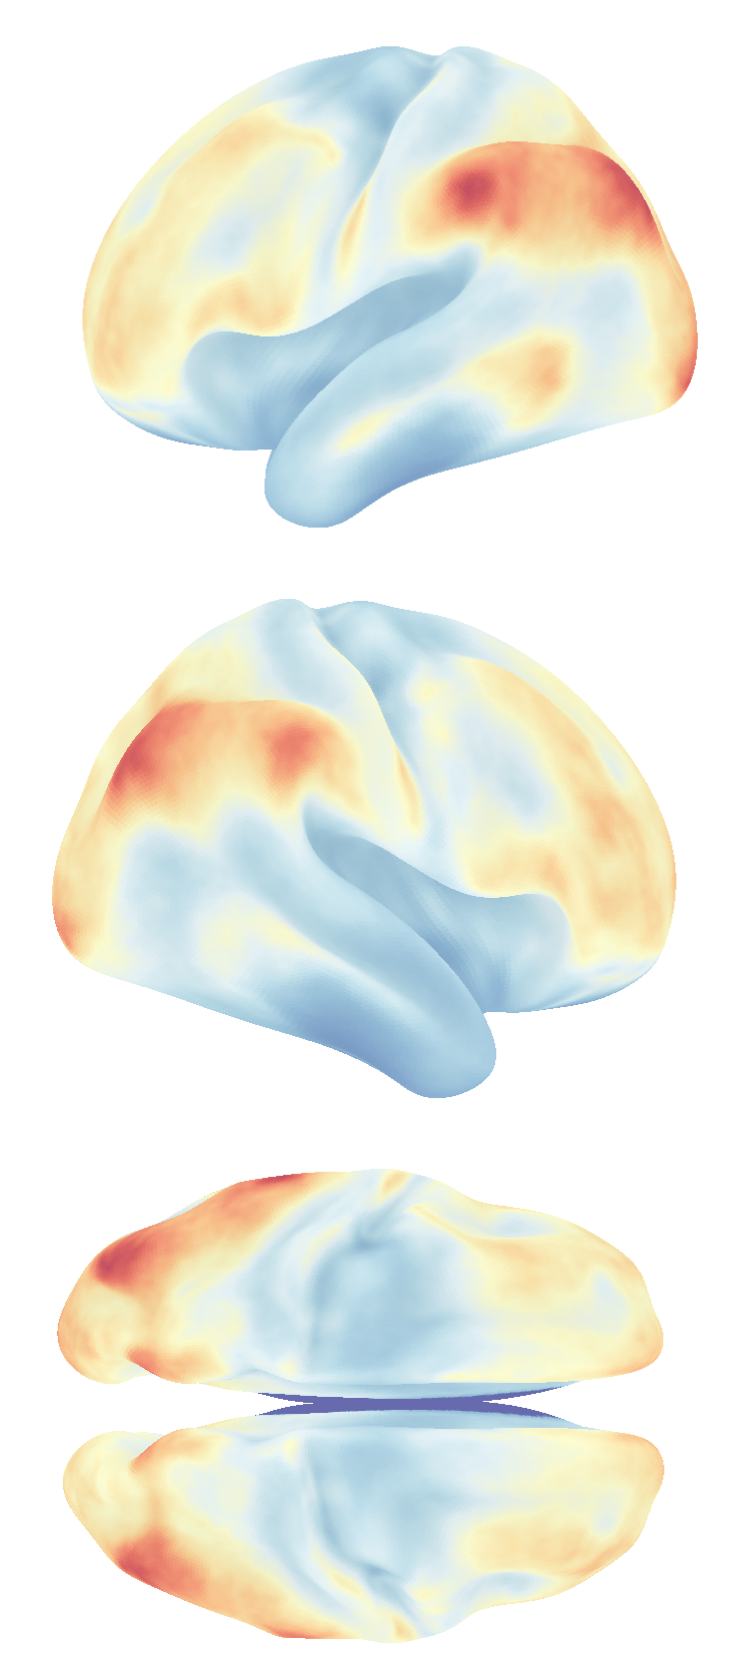
\includegraphics[width=0.5\textwidth]{latex/slides/hcp7T.png}}
\end{columns}
\end{frame}


\section{Motivations}

% slide % 
\subsection{Scientific}
\begin{frame}{Scientific Motivation}
\footnotesize

Neural timeseries often exhibit time-lagged correlation, or temporal receptive fields, that are characterized by an autocorrelation function that decays exponentially with time.\\
\vspace{.5cm}
Timescale parameters control the autocorrelation function decay rate (\cite{gao_neuronal_2020})

\visible{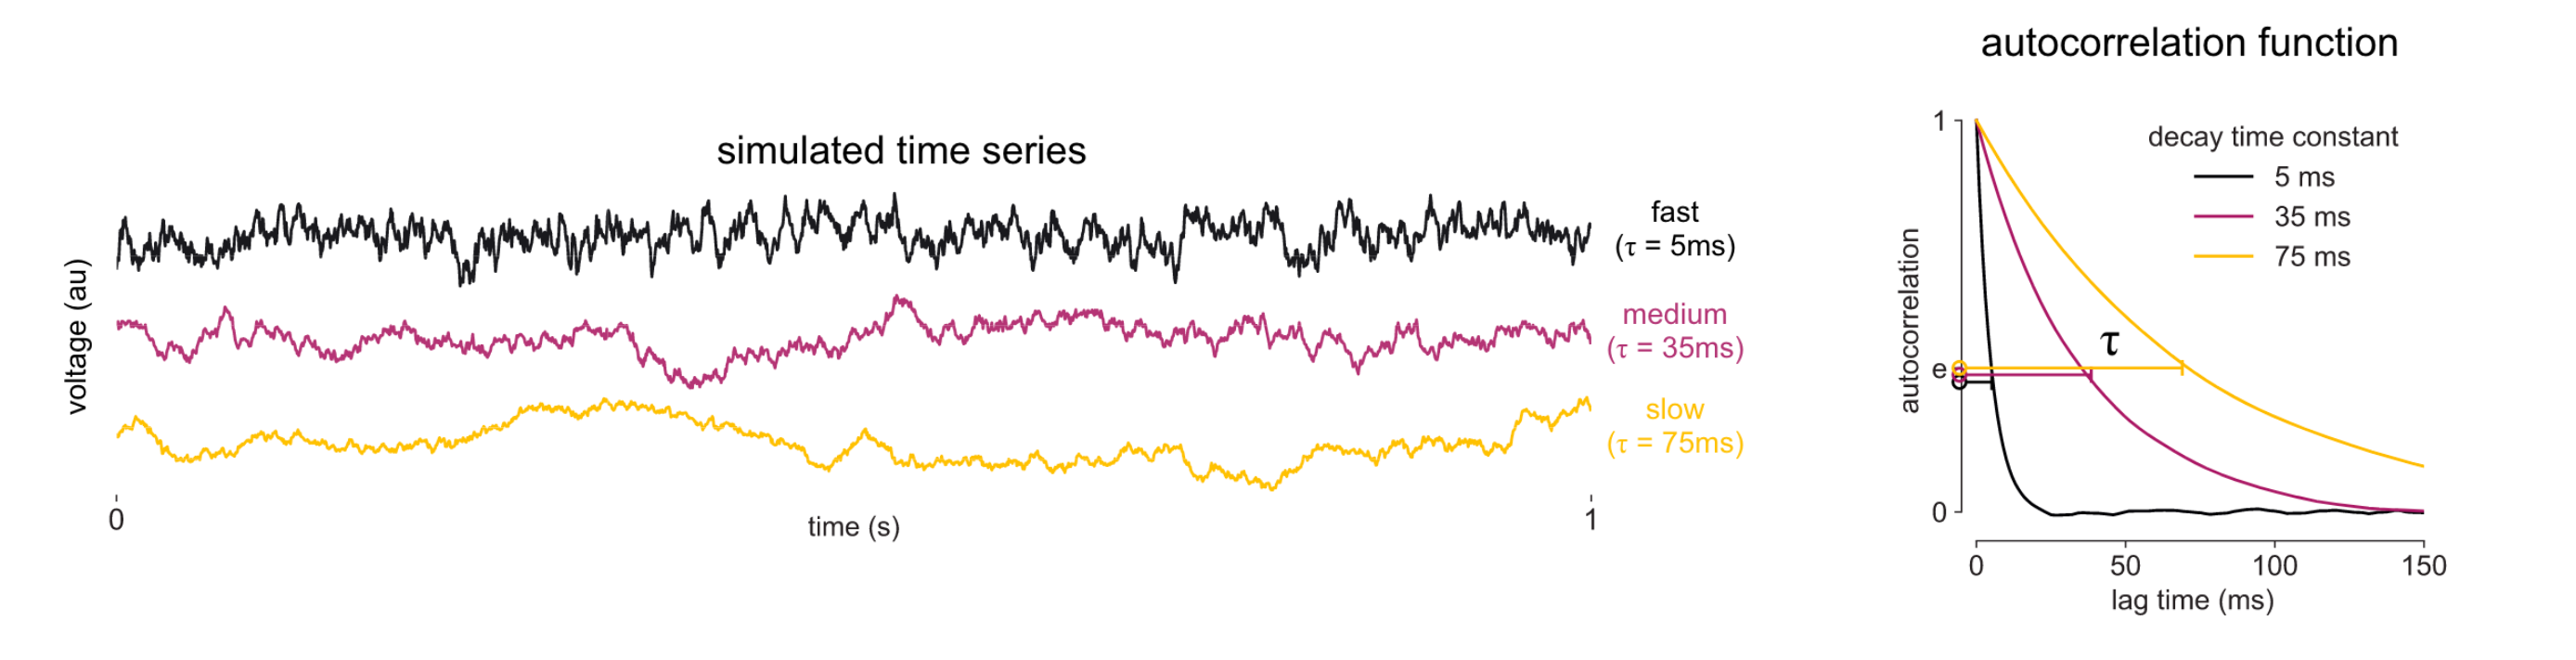
\includegraphics[width=0.95\textwidth]{latex/slides/gao-et-al.png}}
\end{frame}

% slide %
\begin{frame}{Timescale Organization}
\footnotesize
Timescales follow a hierarchy from sensory to associative regions of cortex (\cite{murray_hierarchy_2014}).
\visible{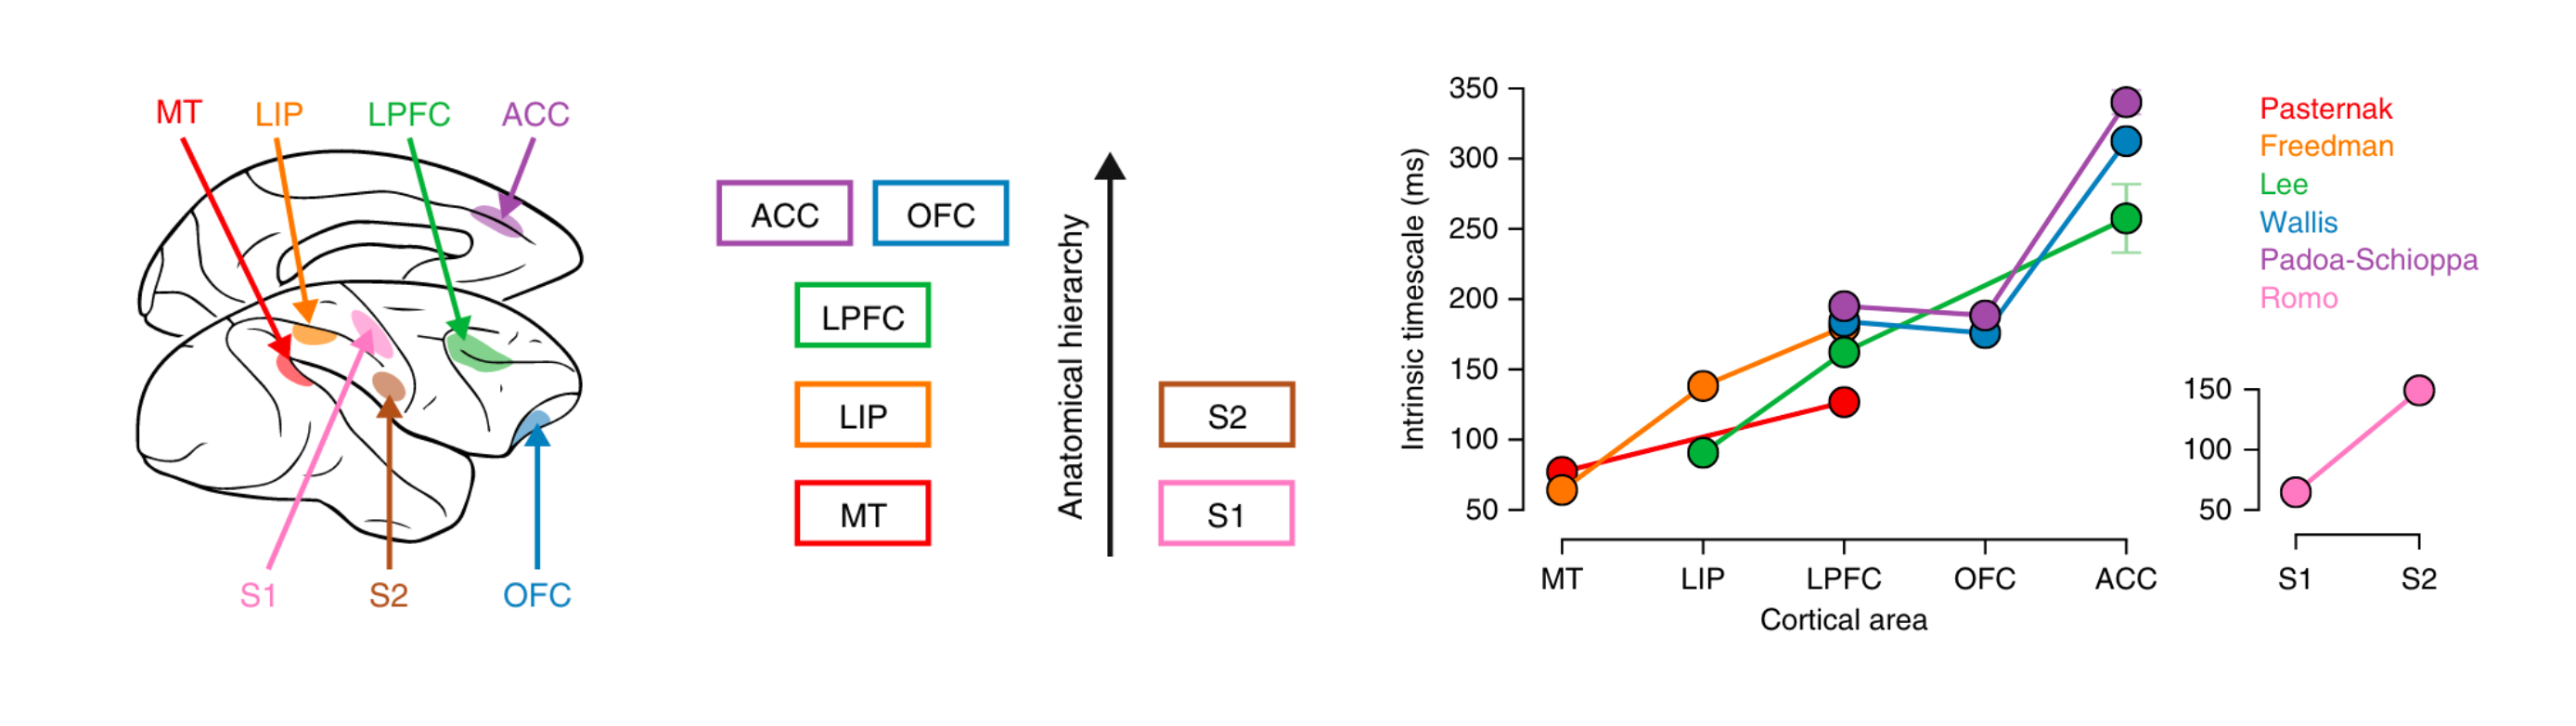
\includegraphics[width=0.95\textwidth]{latex/slides/murray-et-al.png}}

This pattern repeats itself in subcortical regions (\cite{raut_hierarchical_2020, muller_core_2020, nougaret_intrinsic_2021}).
\visible{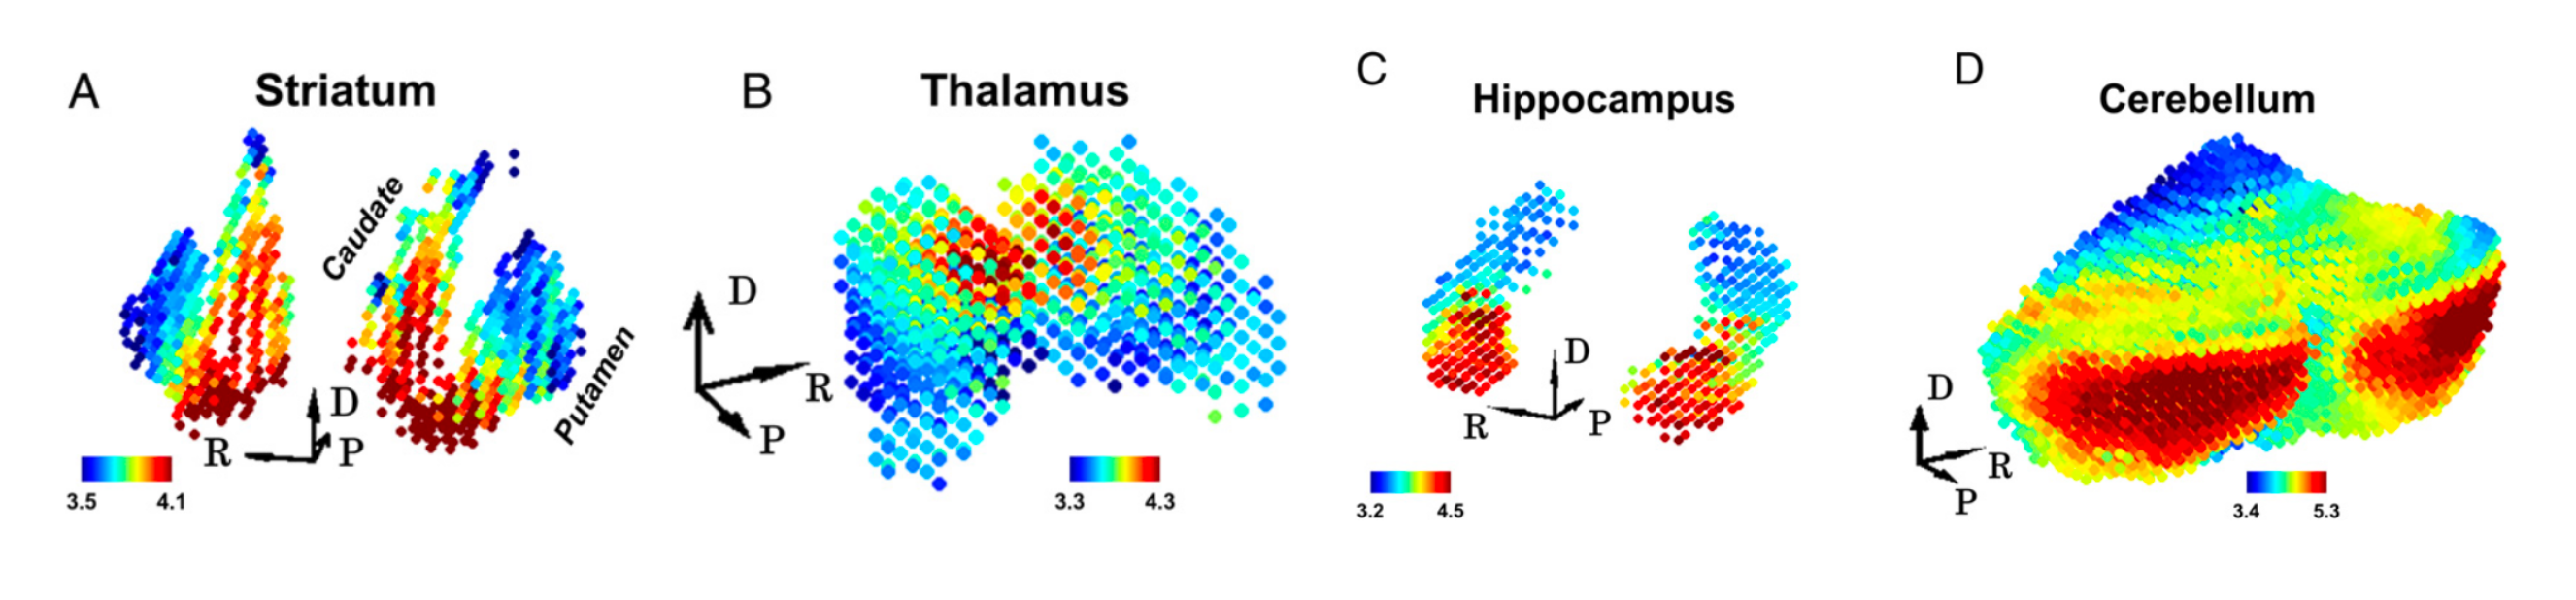
\includegraphics[width=0.95\textwidth]{latex/slides/raut-et-al.png}}
\end{frame}

% slide %
\begin{frame}{Timescale Function}
\footnotesize
Timescales have functional importance:\\ 
\vspace{0.25cm}
\textbf{experimental conditions}
\begin{itemize}
    \item Pharmacological agents: Propofol \cite{huang_timescales_2018} and Serotonergic drugs (\cite{shinn_functional_2023})
    \item Working memory tasks (\cite{gao_neuronal_2020})
    \item Sleep deprivation (\cite{meisel_decline_2017})
\end{itemize}
\vspace{0.25cm}
\textbf{observational studies}
\begin{itemize}
    \item Ageing (\cite{gao_neuronal_2020})
    \item Psychiatric disorders: Autism (\cite{watanabe_atypical_2019}) and Schizophrenia (\cite{wengler_distinct_2020})
\end{itemize}
\end{frame}

% slide % 
\begin{frame}{Imaging Modalities}
\centering
\visible{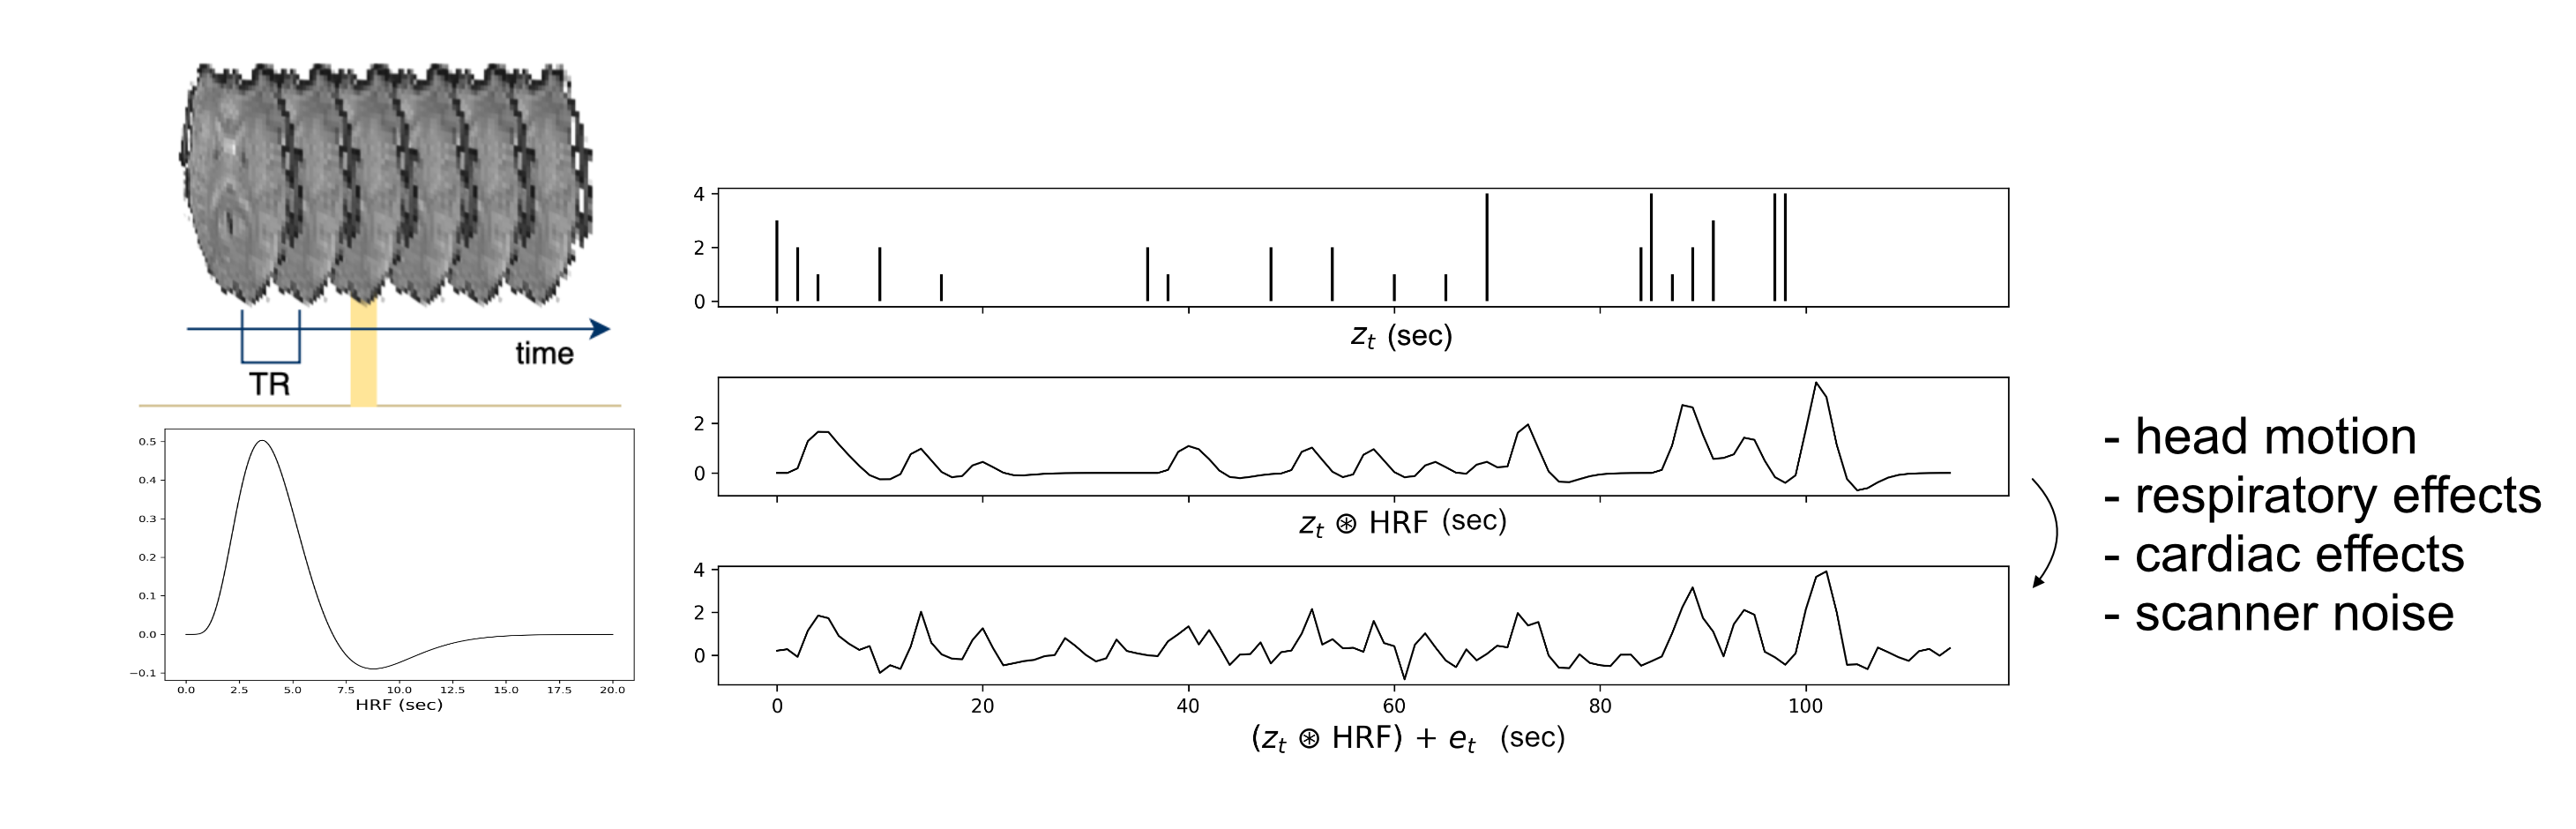
\includegraphics[width=0.95\textwidth]{latex/slides/hrf.png}}
\end{frame}

% slide % 
\begin{frame}{Functional MRI}
\centering
\visible{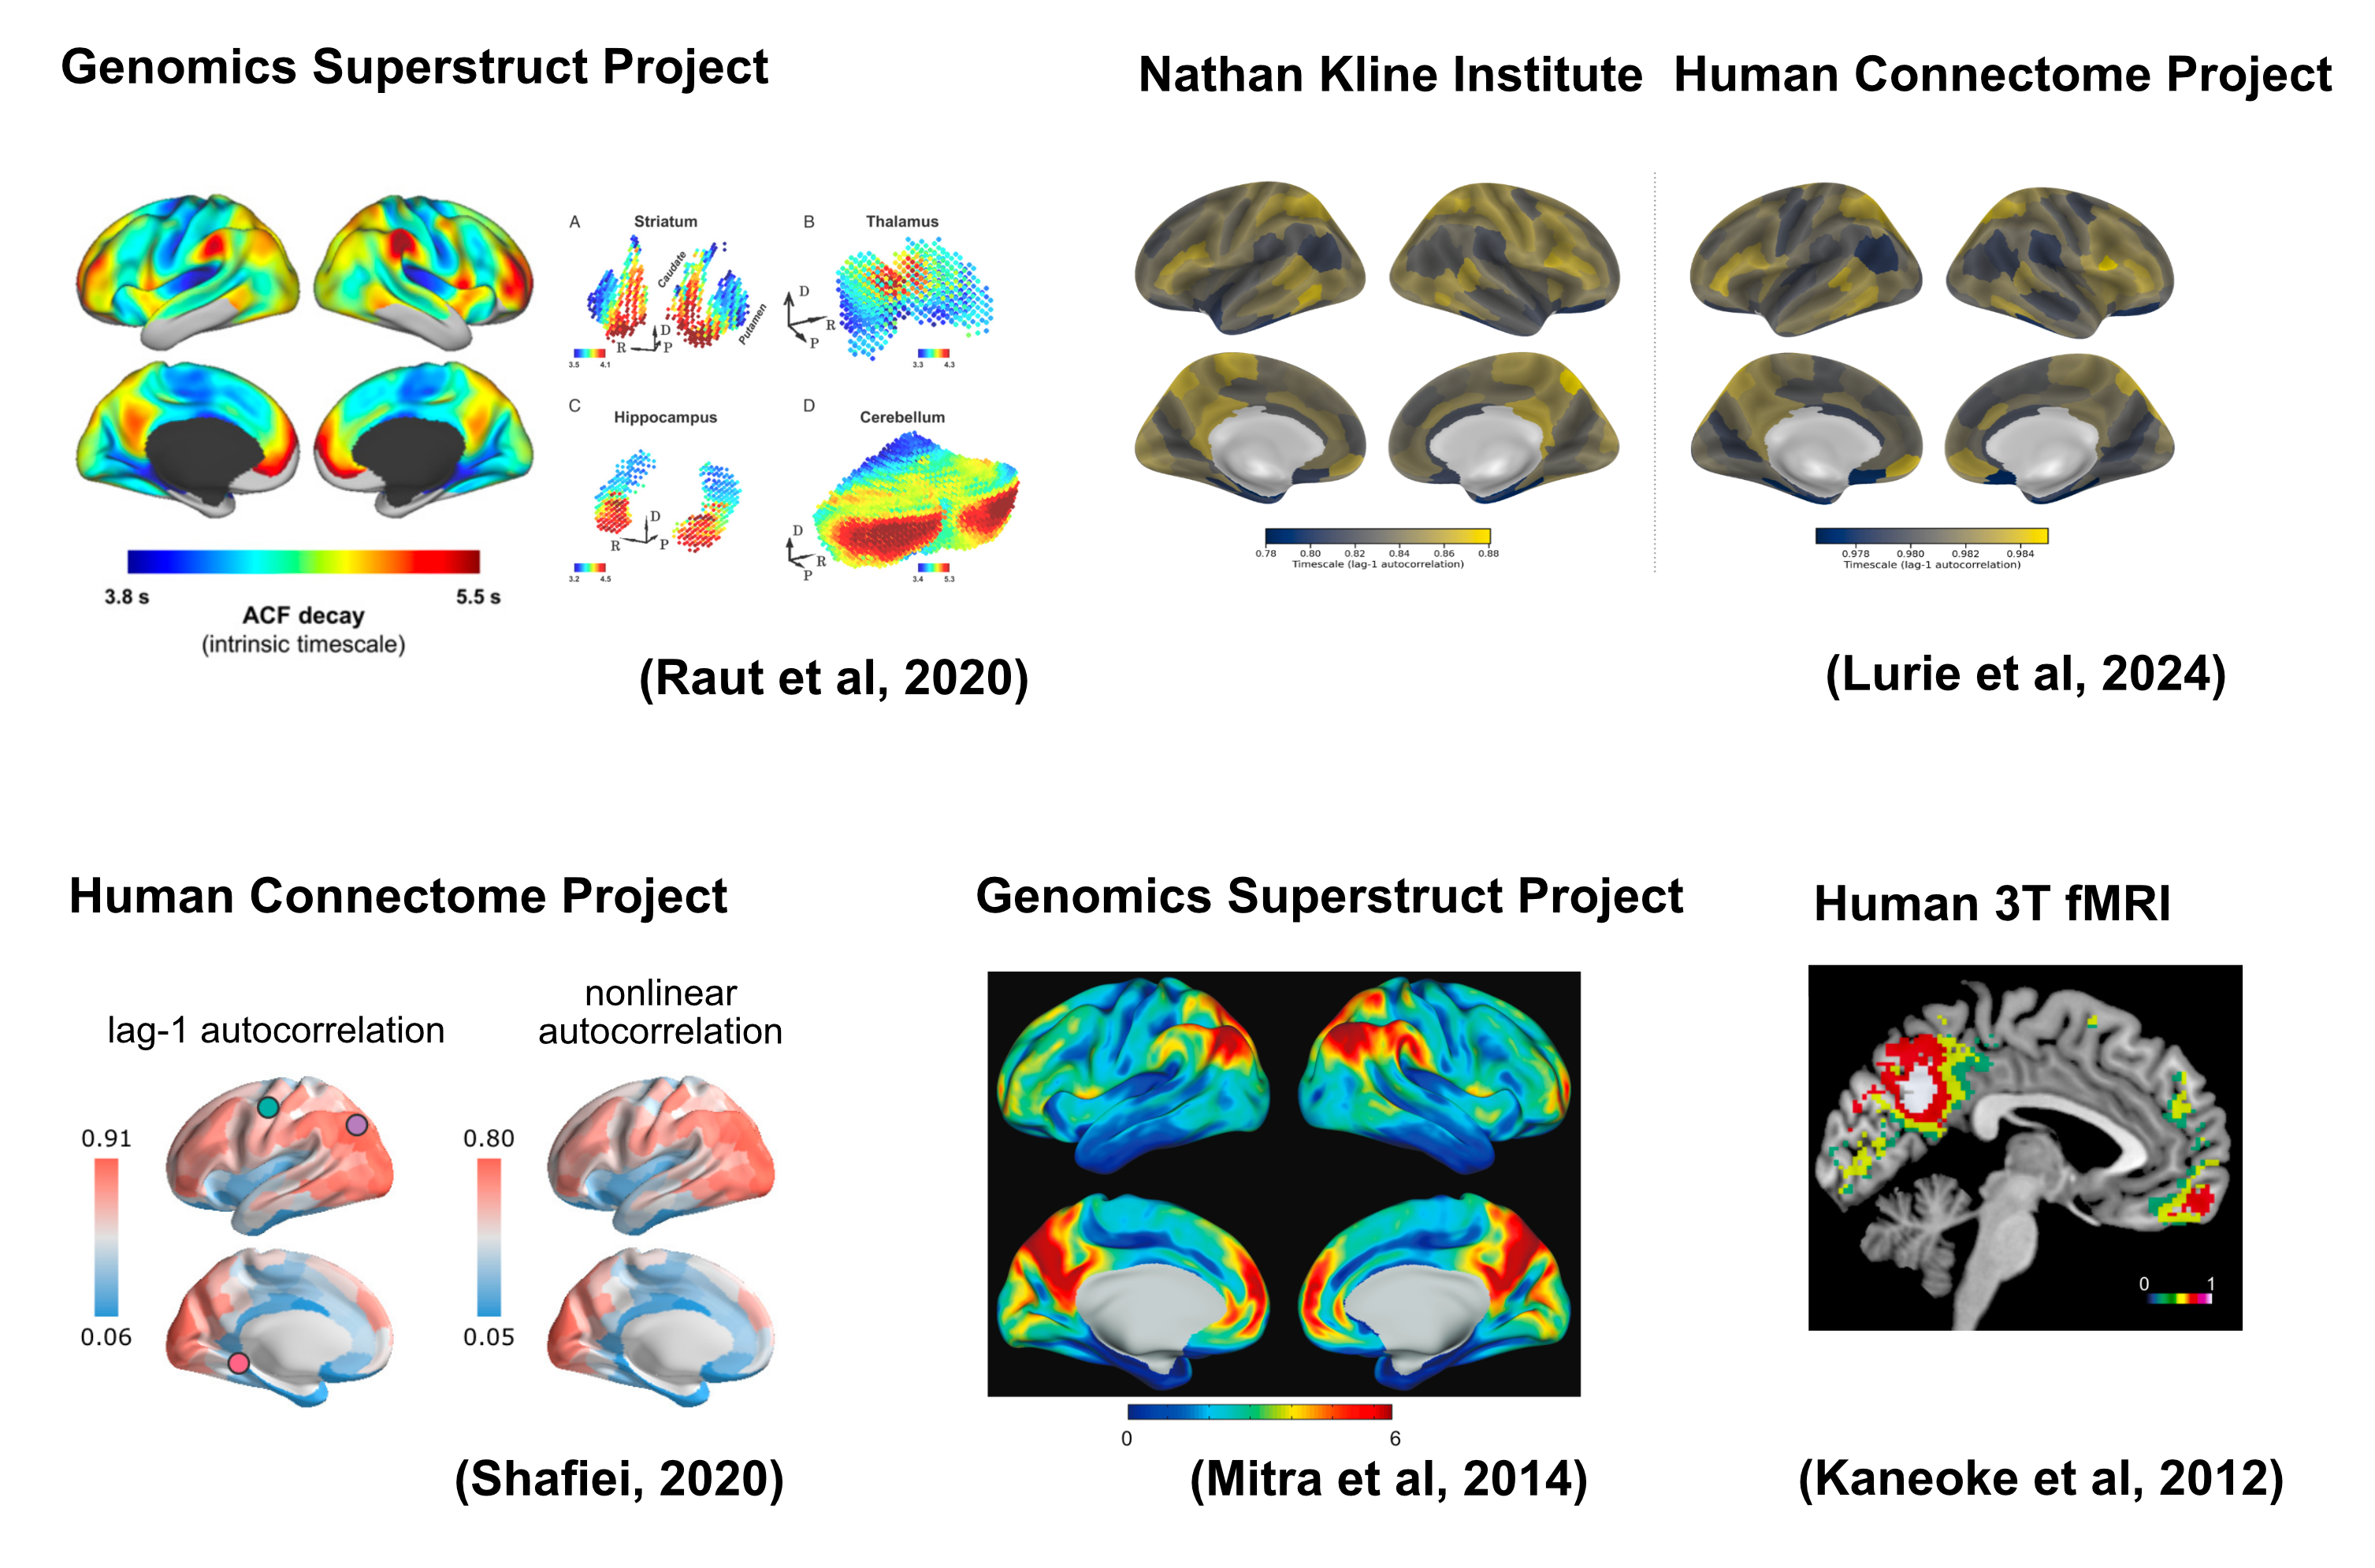
\includegraphics[width=0.95\textwidth]{latex/slides/fmri-maps01.png}}
\scriptsize
\cite{raut_hierarchical_2020, lurie_cortical_2024, shafiei_topographic_2020, mitra_lag_2014, kaneoke_variance_2012}
\end{frame}

% slide %
\begin{frame}{Functional MRI}
\centering
\visible{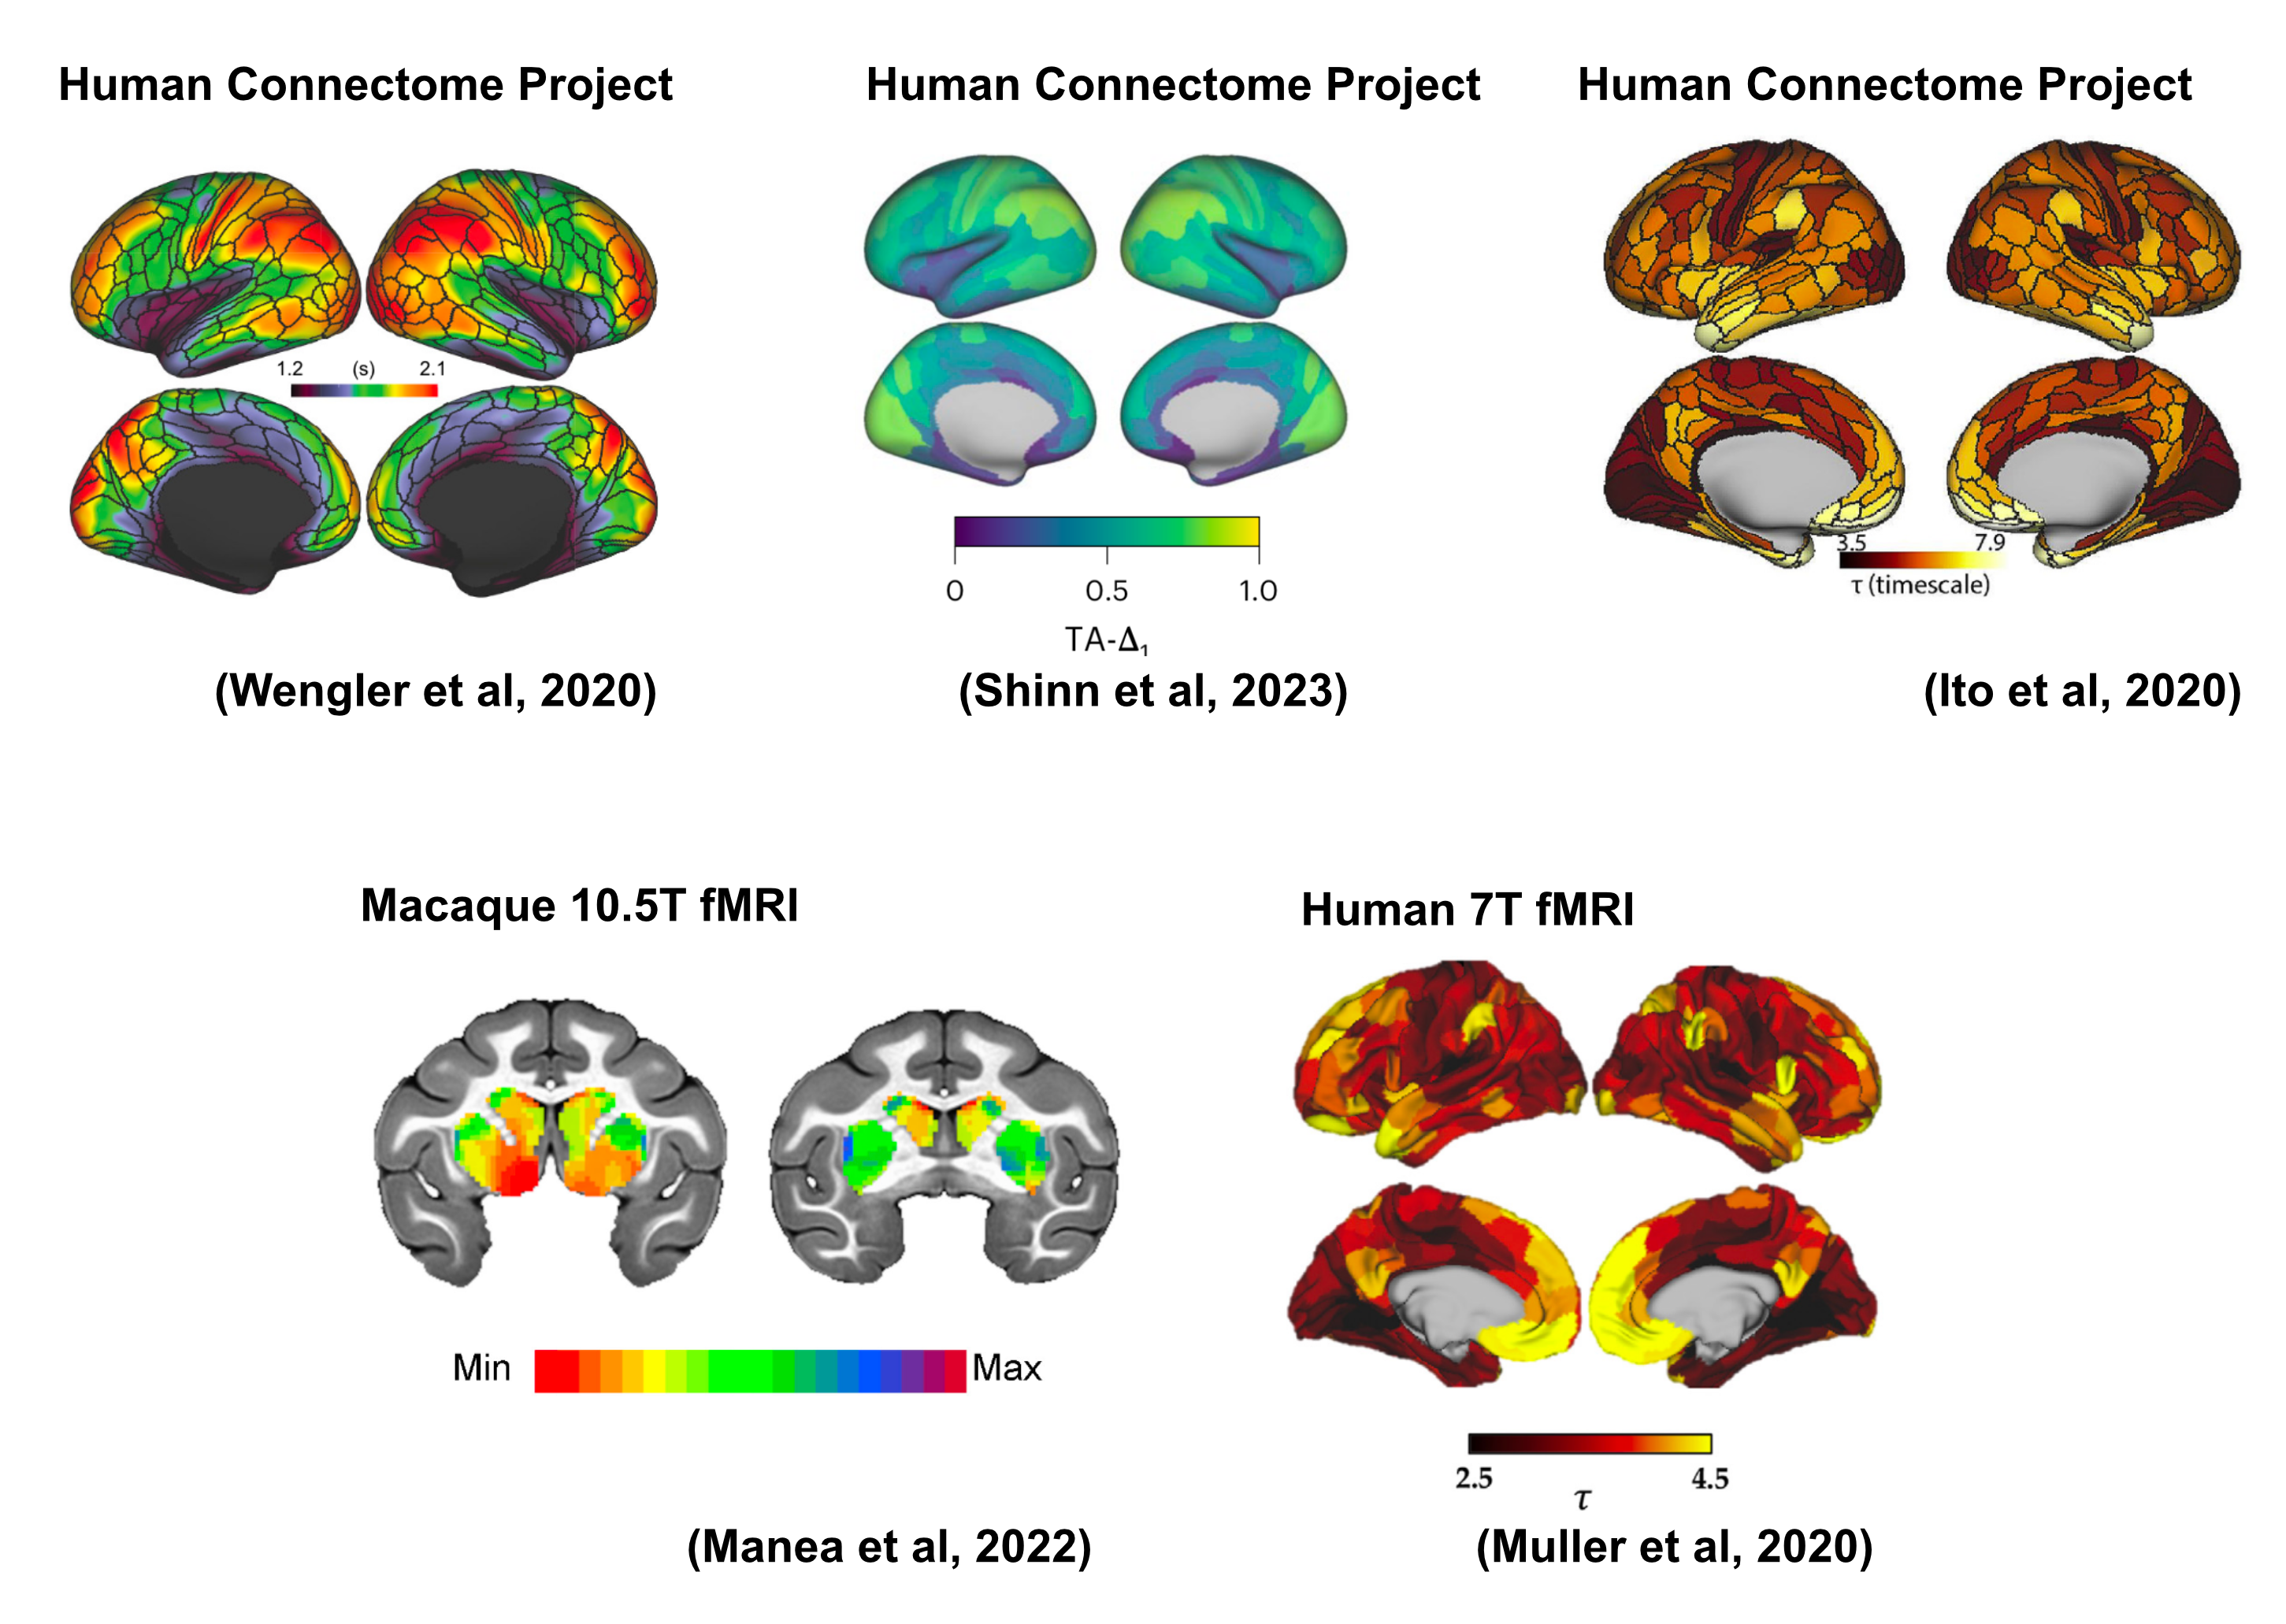
\includegraphics[width=0.95\textwidth]{latex/slides/fmri-maps02.png}}
\scriptsize
\cite{wengler_distinct_2020, shinn_functional_2023, ito_cortical_2020, manea_intrinsic_2022, muller_core_2020}
\end{frame}

% slide %
\subsection{Methodological}
\footnotesize
\begin{frame}{Methodological Motivation}
\begin{enumerate}
    \item \textbf{Time Domain} (6/25 papers):\\
    \begin{scriptsize}
        \cite{kaneoke_variance_2012, meisel_decline_2017, huang_timescales_2018, lurie_cortical_2024, shinn_functional_2023, shafiei_topographic_2020}
    \end{scriptsize}
    \item \textbf{Autocorrelation Domain} (18/25 papers):\\
    \begin{scriptsize}
        \cite{murray_hierarchy_2014, rossi-pool_invariant_2021, cirillo_neural_2018, ito_cortical_2020, runyan_distinct_2017, zeraati_flexible_2022, nougaret_intrinsic_2021, wasmuht_intrinsic_2018, muller_core_2020, maisson_choice-relevant_2021, li_hierarchical_2022, shafiei_topographic_2020, wengler_distinct_2020, manea_intrinsic_2022, watanabe_atypical_2019, zilio_are_2021, raut_hierarchical_2020, golesorkhi_temporal_2021}
    \end{scriptsize}
    \item \textbf{Frequency Domain} (3/25 papers):\\
    \begin{scriptsize}
        \cite{gao_neuronal_2020, zeraati_flexible_2022, fallon_timescales_2020}
    \end{scriptsize}
\end{enumerate}
\end{frame}

\section{Definitions}

% slide %
\subsection{Assumptions}
\begin{frame}{Assumptions}
\end{frame}

% slide %
\subsection{Models}
\begin{frame}{Exponential Decay Model}
\scriptsize

\textbf{Def. Autocorrelation Function}:
\begin{align}
    \rho_k = \text{corr}(X_t, X_{t-k}) = \frac{\gamma_k}{\gamma_0}
\end{align}

\onslide<2->
\textbf{Def. Exponential Decay Model}:
\begin{align} \label{eq:acf}
\rho_k &= \text{exp}(-\frac{k}{\tau}) + e_k
\end{align}

\onslide<3->
\textbf{Def. Timescale}: 
\begin{align}
    L(\tau) &= \mathbb{E}[(\rho_k - \text{exp}(-\frac{k}{\tau}))^2]\\
    \tau^* &= \underset{\tau}{\text{argmin }} L(\tau)
\end{align}

\end{frame}

\begin{frame}{Autoregressive Model}
\scriptsize

\textbf{Def. Autocorrelation Model}
\begin{align}
    X_t = \phi X_{t-1} + e_t
\end{align}

\onslide<2->
\textbf{Def. Timescale}
\begin{align}
    \phi &= (\mathbb{E}[X_{t-1}^2])^{-1}(\mathbb{E}[X_t X_{t-1}])\\
    \tau &= g(\phi) = -\frac{1}{\text{log}(|\phi|)}. \label{eq:ar1-tau}
\end{align}
\end{frame}

% slide %
\subsection{Estimators}
\begin{frame}{Estimation of Exponential Decay Model}
\scriptsize

\textbf{Est: Autocorrelation Function}
\begin{align}
    \hat\rho_k &= (\hat\gamma_0)^{-1}(\hat\gamma_k) = (\sum_{t=1}^T x_t^2)^{-1} (\sum_{t=k+1}^{T}x_t x_{t-k})
\end{align}

\onslide<2->
\textbf{Est: Nonlinear Least Squares}
\begin{align}
    \hat L(\tau) &= \frac{1}{K} \sum_{k=1}^K (\hat\rho_k - \text{exp}(-\frac{k}{\tau}))^2\\
    \hat\tau^* &= \underset{\tau}{\text{argmin }} \hat L(\tau)
\end{align}

\onslide<3->
\textbf{Est: Sandwich Standard Error}
\begin{align}
    \hat\sigma^2 &= \frac{1}{K-1} \hat L(\hat\tau^*) \notag\\
    \text{se}_\text{Naive}(\hat\tau^*) &= \sqrt{\hat\sigma^2 (\hat L''(\hat\tau^*))^{-1}}.
\end{align}
\end{frame}

% slide %
\begin{frame}{Estimation of Autoregressive Model}
\scriptsize

\textbf{Est: Linear Least Squares}
\begin{align}
    \hat\phi &= (\sum_{t=2}^T x_{t-1}^2)^{-1} (\sum_{t=2}^T x_t x_{t-1})\\
    \hat\tau &= g(\hat\phi) = -\frac{1}{\text{log}(|\hat\phi|)}
\end{align}

\onslide<2->
\textbf{Est: Sandwhich Standard Error}
\begin{align}
    \hat u_t &= x_{t-1} \hat e_t \notag\\
    \hat \omega &= \sum_{k=-M}^M (1 - \frac{|k|}{M+1}) \sum_{t-k}^T \hat u_t \hat u_{t-k} \notag\\
    \text{se}_{NW}(\hat\phi) &= (\sum_{t=2}^T x_{t-1})^{-1} \quad \hat \omega \quad (\sum_{t=2}^T x_{t-1})^{-1}.
\end{align}

\end{frame}

% slide %
\subsection{Properties}
\begin{frame}{Properties of NLS}
\scriptsize 
\textbf{Consistency}:\\
...\\
\textbf{Limiting Variance}:\\
...\\
\end{frame}


% slide %
\begin{frame}{Properties of LLS}
\scriptsize 
\textbf{Consistency}:\\
...\\
\textbf{Limiting Variance}:\\
...\\
\end{frame}

\section{Simulations}

% side %
\subsection{Settings}
\begin{frame}{AR-1, AR-2, HCP}
\end{frame}

% slide %
\begin{frame}{AR-2 Stationarity Conditions}
\centering
\visible{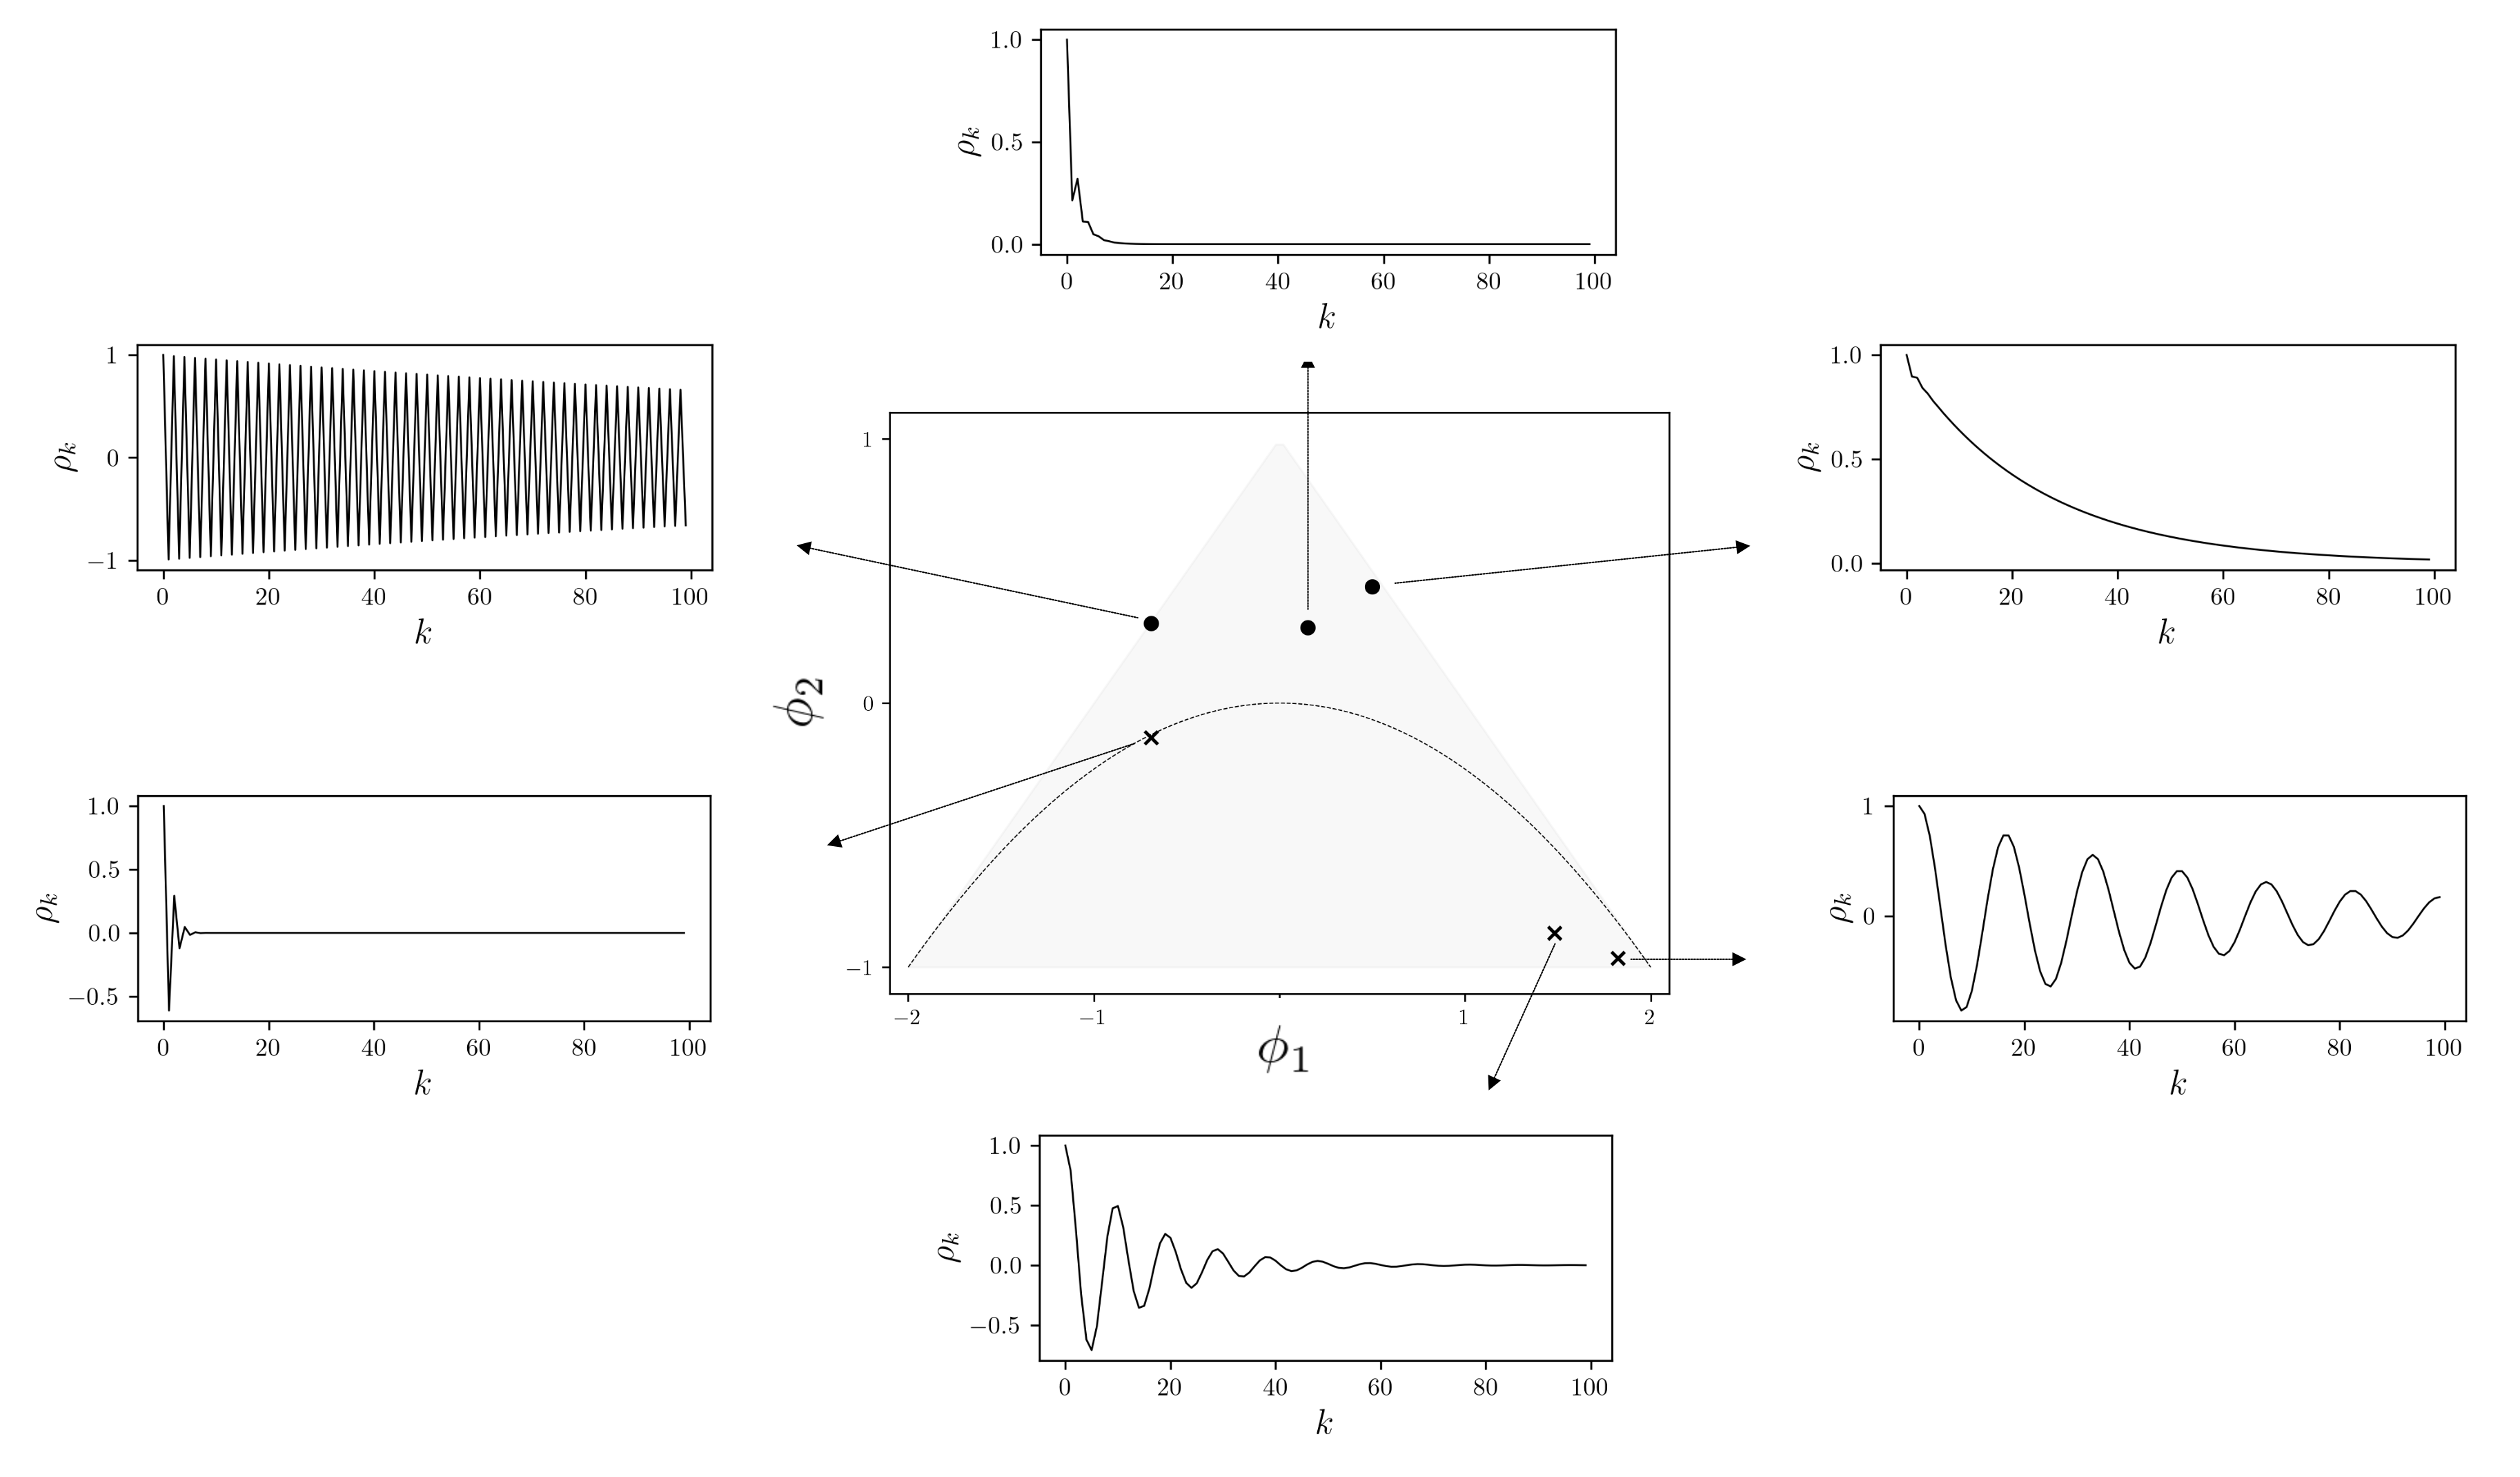
\includegraphics[width=0.99\textwidth]{latex/slides/ar2-stationary-triangle.png}}
\end{frame}

% slide %
\begin{frame}{AR-2 Stationarity Conditions}
\centering
\visible{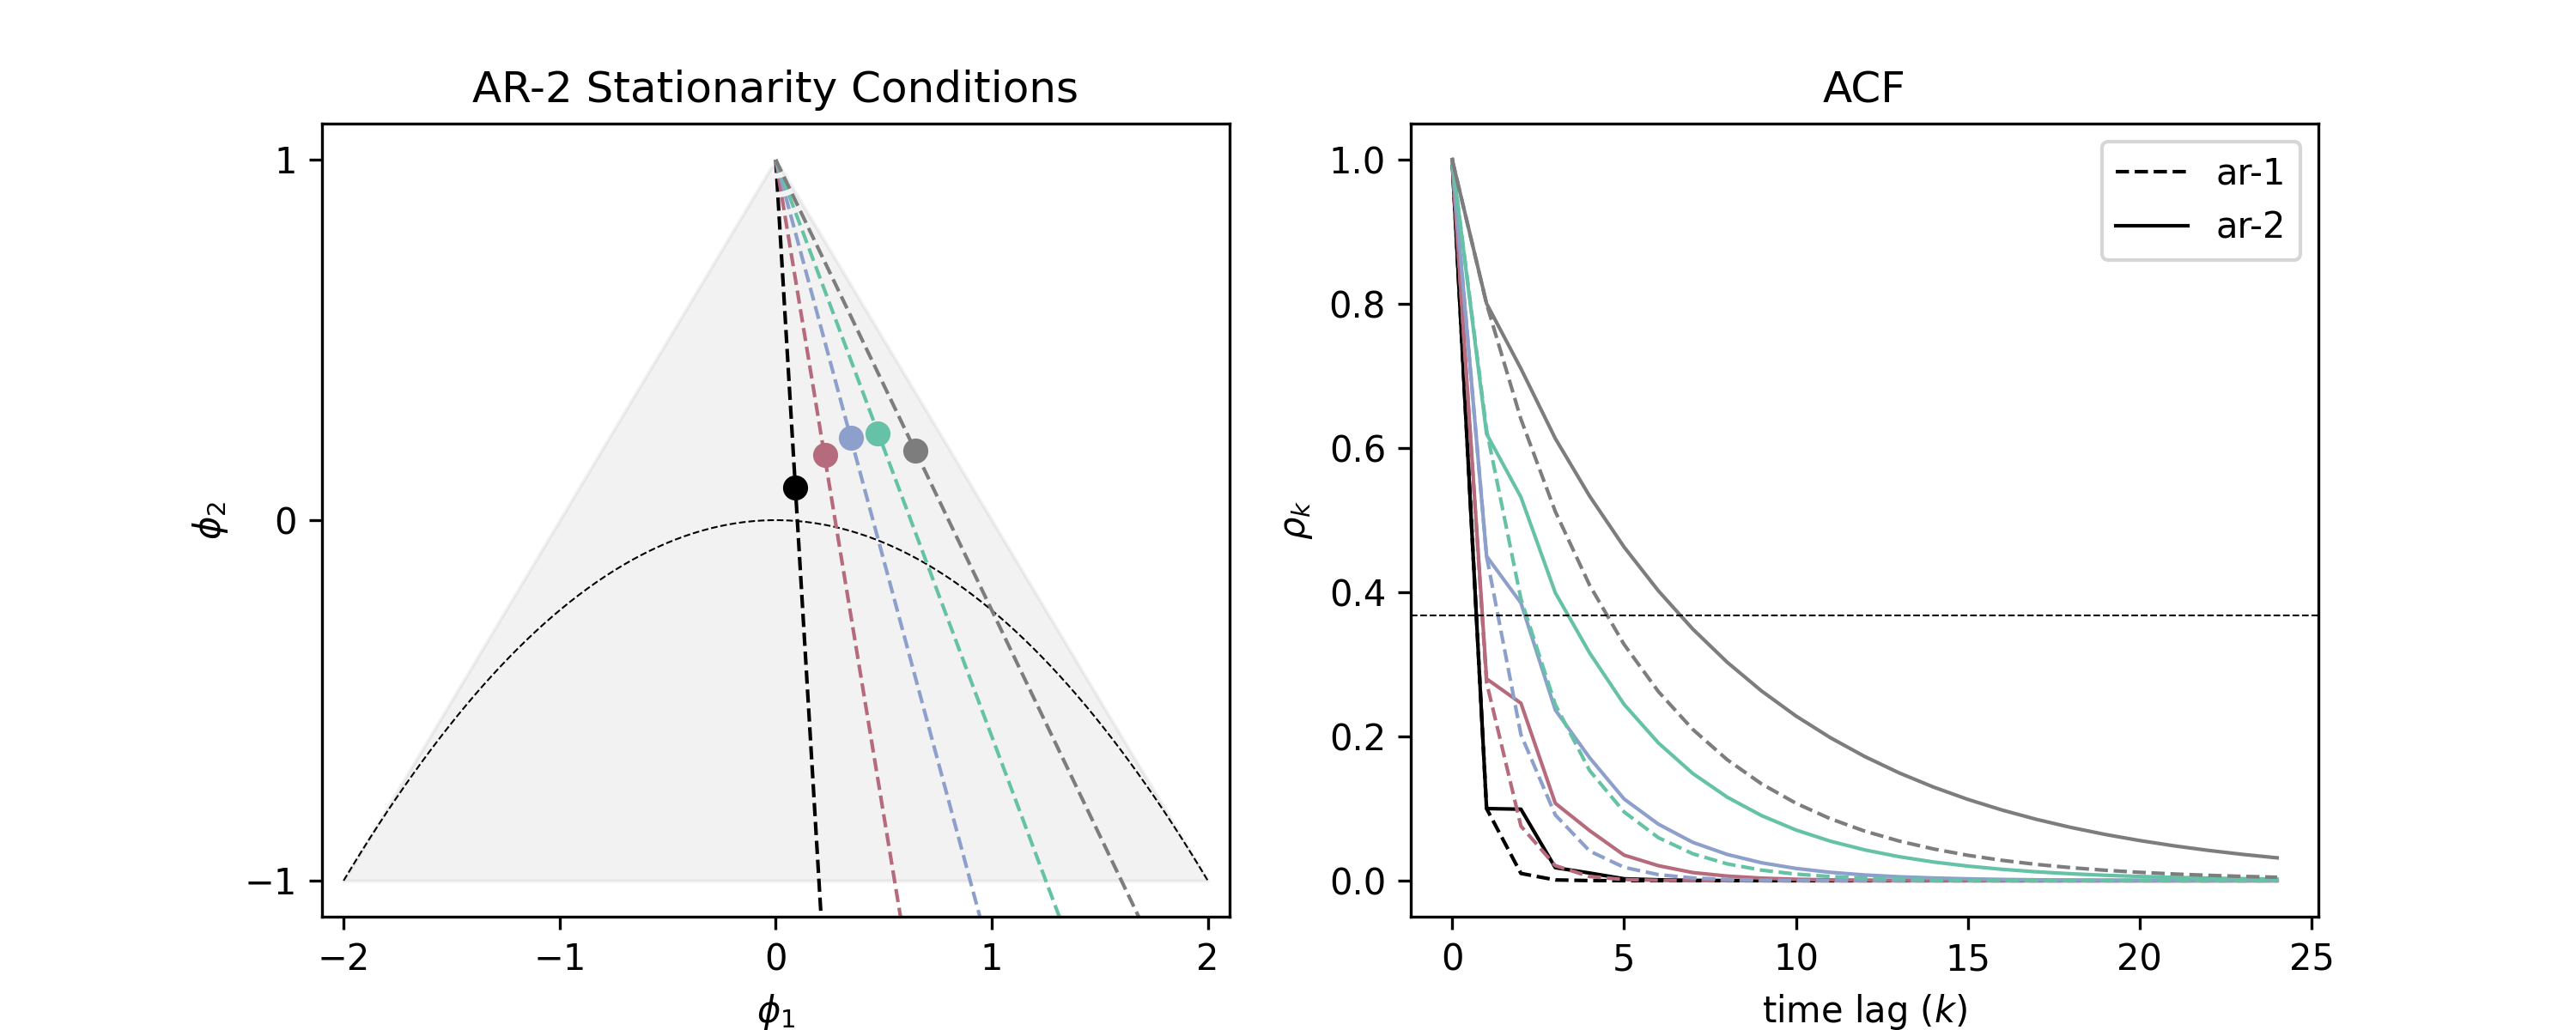
\includegraphics[width=0.99\textwidth]{latex/slides/simulations-ar2.png}}
\end{frame}

% slide %
\subsection{Results}
\begin{frame}{AR(1) Results}
\end{frame}

% slide %
\begin{frame}{AR(2) Results}
\end{frame}

% slide %
\begin{frame}{HCP Results}
\end{frame}

\section{Applications}

% slide %
\subsection{Dataset Description}
\begin{frame}{Dataset Description}
    \centering
    \visible{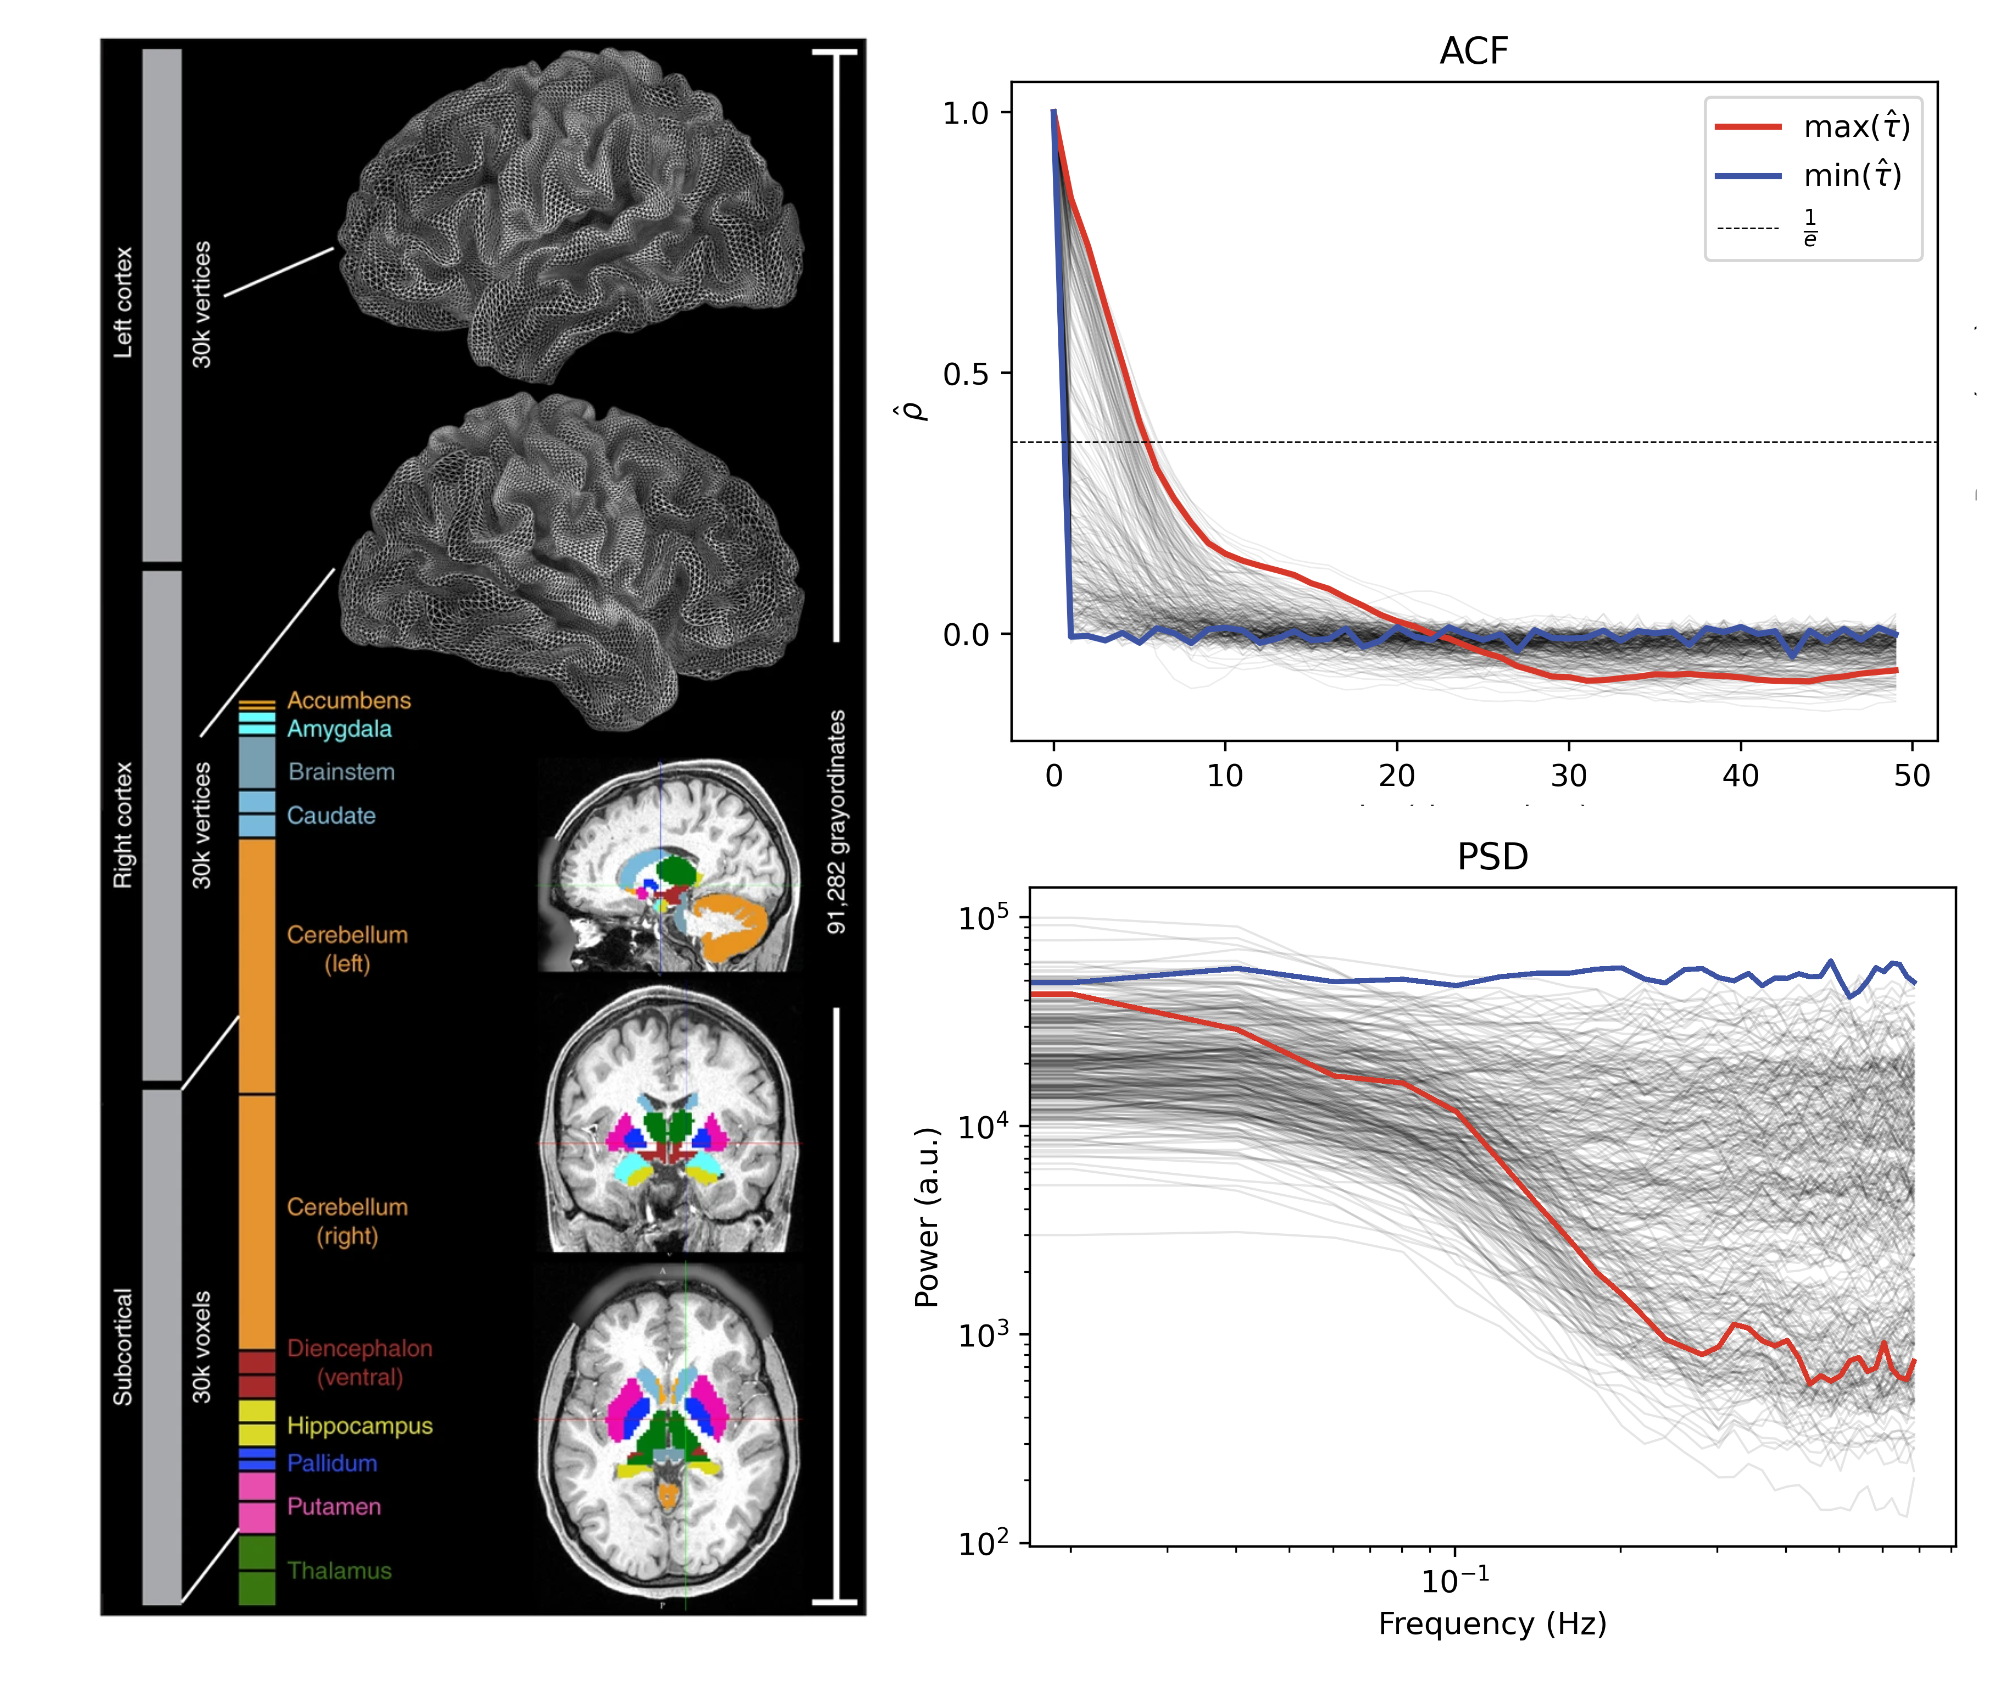
\includegraphics[width=0.85\textwidth]{latex/slides/dataset-description.png}}
    \scriptsize
    \begin{enumerate}
    \item Developing Methods: 10 subjects, 4800 timepoints, 300 regions
    \item \textbf{Estimating Maps:  184 subjects, 3600 timepoints, 91282 grayordinates}
    \end{enumerate}
\end{frame}

% slide %
\subsection{Timescale Maps}
\begin{frame}{Timescale Maps}
\scriptsize
$\hat \tau_{LLS}$
\visible{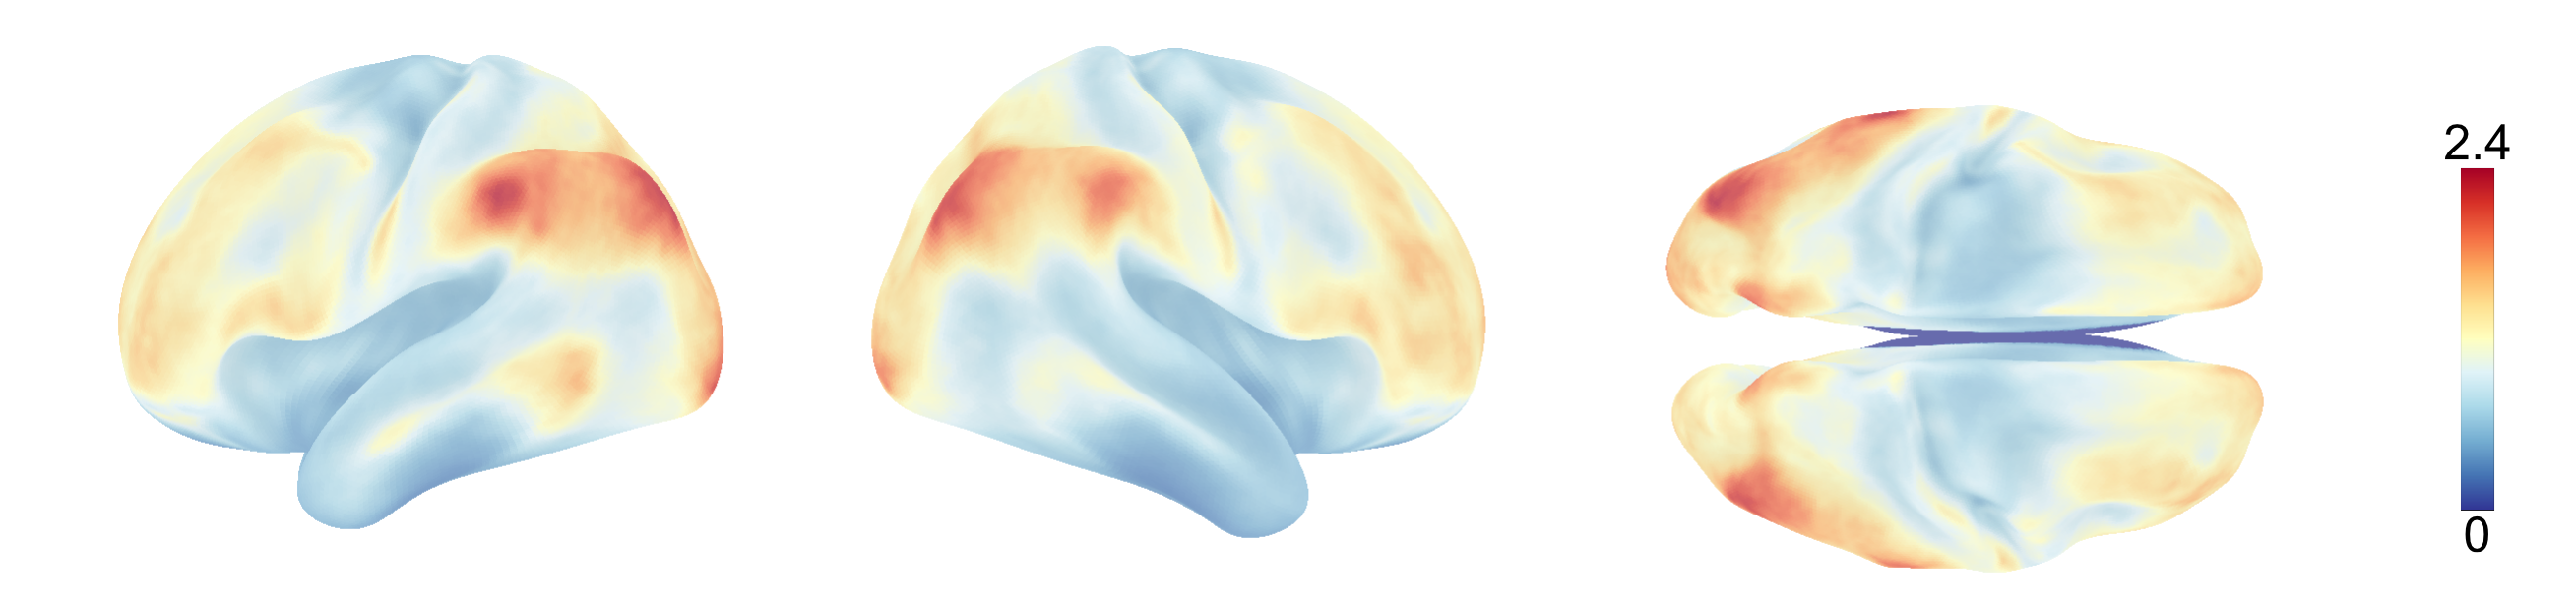
\includegraphics[width=1\textwidth]{latex/slides/tau_map.png}}
$\text{se}_{NW}(\hat \tau)$
\visible{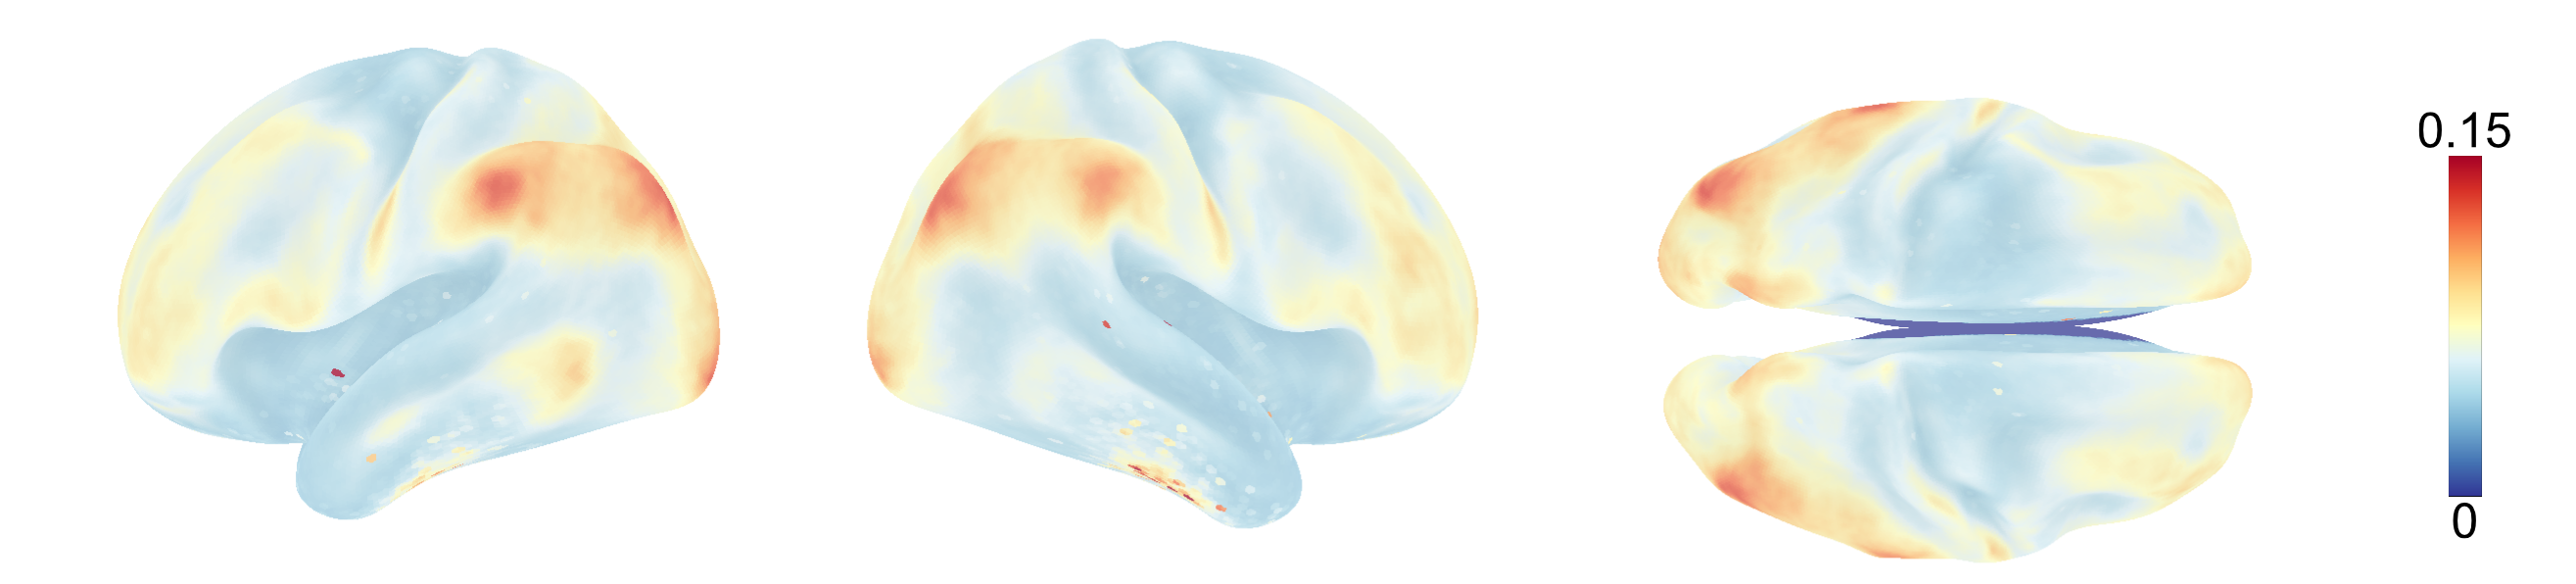
\includegraphics[width=1\textwidth]{latex/slides/se_map.png}}
$(\hat \tau_{LLS} - 1) / \text{se}_{NW}(\hat \tau)$
\visible{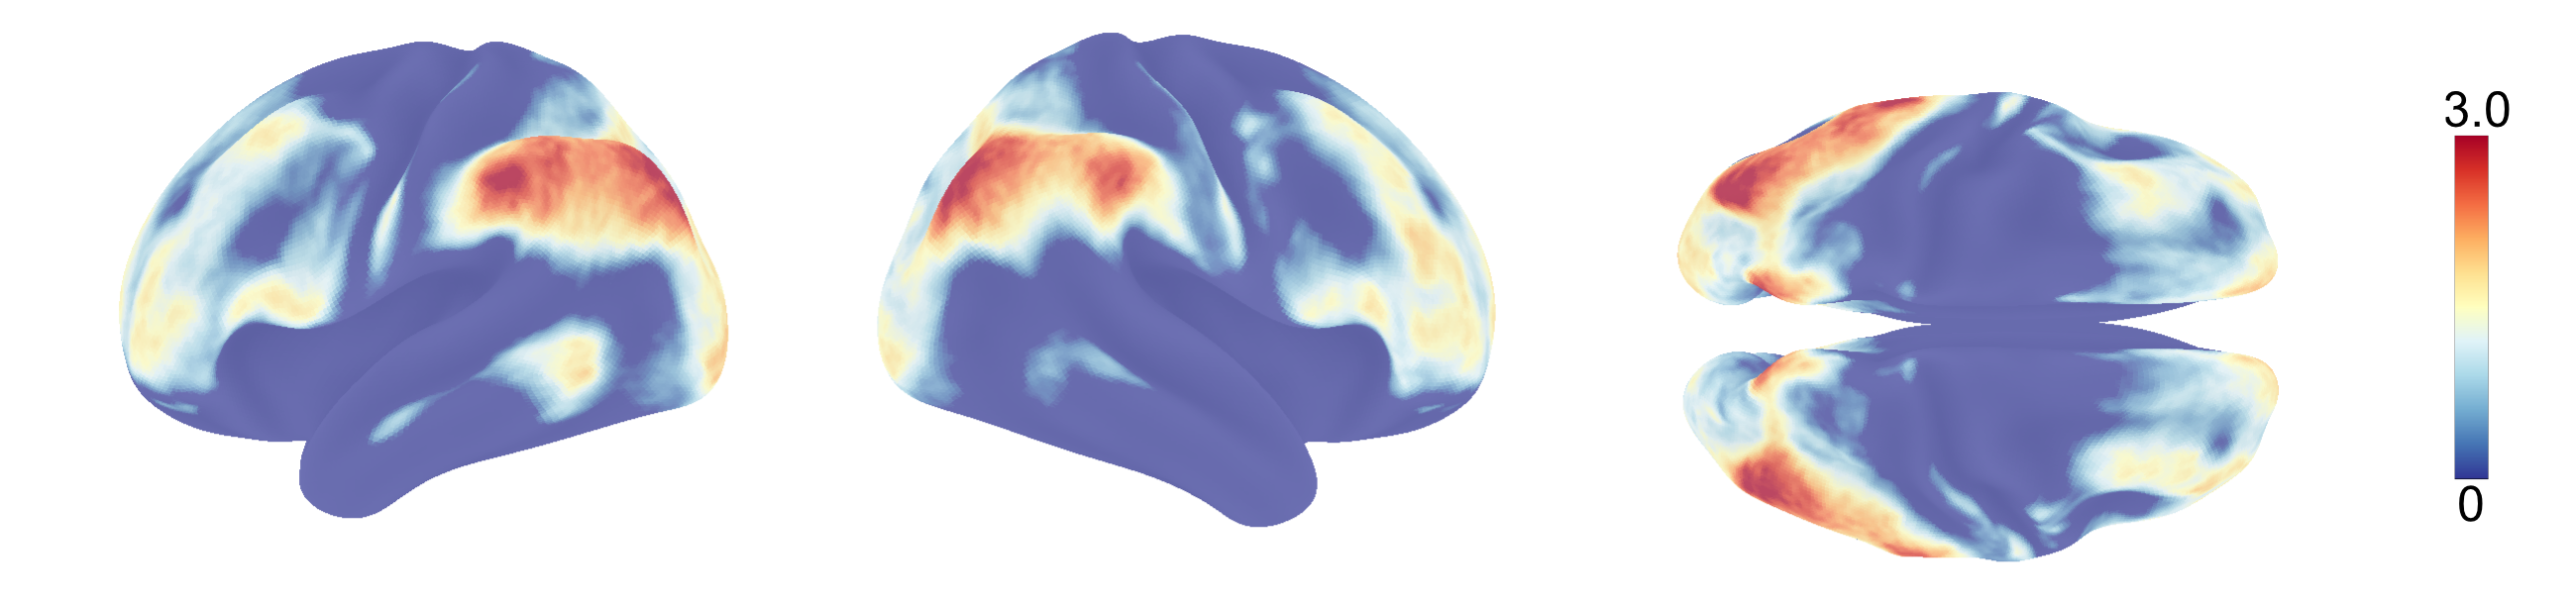
\includegraphics[width=1\textwidth]{latex/slides/tstat_map.png}}
\end{frame}

% slide %
\section{Conclusions}
\begin{frame}{Conclusions and Future Directions}
\end{frame}

% slide %
\section{References}
\begin{frame}{References}
\end{frame}

\end{document}